%
% kmatrix.tex
%
% (c) 2018 Prof Dr Andreas Müller, Hochschule Rapperswil
%
\subsection{Kamera-Spezifikation\label{section:kameraspez}}
Die im Abschnitt~\ref{section:homogene koordinaten} beschriebene
Lösung des Abbildungsproblems bildet die Punkte auf der Kameraachse
auf den Nullpunkt der Brennebene ab.
Der Chip einer realen Kamera ist dagegen nur ein Rechteck, 
welches üblicherweise mit einem Koordinatensystem ausgestattet wird,
welches den Nullpunkt in einer Ecke hat.
Als Masseinheit werden ausserdem meistens Pixel verwendet, nicht die
Masseinheiten, die für Weltpunkte verwendet werden.
Dieser Chip wird meistens so montiert, dass die Achse der Kamera
durch den Mittelpunkt des Chips geht.
Wir brauchen daher eine Umrechnungsformel, welche die homogenen
Koordinaten des Bildpunktes in die Chip-Koordinaten umrechnet.

\subsubsection{Brennweite und Pixelkoordinaten}
\begin{figure}
\centering
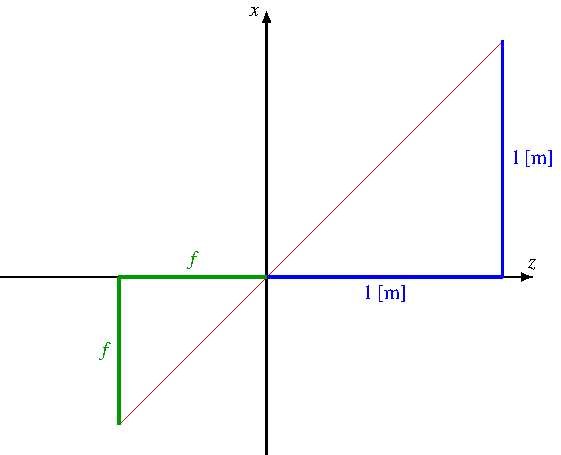
\includegraphics{applications/kamera/brennweite.pdf}
\caption{Brennweite und Umrechnung in Pixelkoordinaten (siehe Text)
\label{skript:kamera:brennweite}}
\end{figure}
Zunächst untersuchen wir nochmals die Bedeutung der Brennweite $f$.
Die Kamera bildet den Punkt $(x,y,z)$ zunächst auf die homogenen
Koordinaten $(x,y,z)$ ab.
Zur Bestimmung der inhomogenen Koordinaten in der Brennebene 
berechnen wir zunächst $(x/z, y/z)$.
Dies entspricht der Projektion in die Brennebene mit $z=1$,
dies gilt aber für $z$ gemessen in den Masseinheiten des
Weltkoordinatensystems.
Wir brauchen nun aber die Umrechnung in Pixel-Koordinaten im Bild,
und verwenden dazu die Abbildung~\ref{skript:kamera:brennweite}.
Wir lesen daraus ab, dass ein Punkt mit homogener Koordinate $(1,1)$
abgebildet wird auf einen Punkt mit inhomgenen Pixelkoordinaten $f$
abgebildet.

In drei Dimensionen bedeutet das, dass der Punkt mit Koordinaten
$(x,y,z)$ abgebildet wird auf den Punkt
\[
(x,y,z) \mapsto (f\cdot x/z, f\cdot y/z).
\]
In Matrixschreibweise ist dies die Folge von Abbildungen
\[
\begin{pmatrix}
x\\y\\z
\end{pmatrix}
\mapsto
\begin{pmatrix}
x/z\\y/z
\end{pmatrix}
\mapsto
\begin{pmatrix}
f\cdot x/z\\f\cdot y/z
\end{pmatrix}.
\]
Die erste Abbildung lässt sich nicht als Matrix schreiben.
Wir könnten aber auf die Divison verzichten und stattdessen
die dritte Komponente $z$ behalten und erst am Schluss durch $z$
dividieren:
\[
\begin{pmatrix}
x\\y\\z
\end{pmatrix}
\mapsto
\begin{pmatrix}
f\cdot x\\f\cdot y\\z
\end{pmatrix}
=
\begin{pmatrix}
f&0&0\\
0&f&0\\
0&0&1
\end{pmatrix}
\begin{pmatrix}
x\\y\\z
\end{pmatrix}
\mapsto
\begin{pmatrix}
f\cdot x/z\\f\cdot y/z
\end{pmatrix}.
\]
Die Skalierung mit der Brennweite wird also am besten mit Hilfe der
Matrix
\[
K_f
=
\begin{pmatrix}f&0&0\\0&f&0\\0&0&1\end{pmatrix}
\]
in homogenen Koordinaten beschrieben.

\subsubsection{Kameraachse und Verschiebung}
Die Achse der Kamera geht durch den Mittelpunkt $(m_x,m_y)$ des Chips.
Punkte der Achse haben homogenen Koordinaten $(0,0,z)$, sollten aber
auf $(m_x,m_y)$ abgebildet werden.
Wir müssen also den inhomogenen Koordinaten noch die Komponenten
$m_x$ und $m_y$ hinzufügen, nämlich
\[
\begin{pmatrix} x/z \\ y/z \\ 1 \end{pmatrix}
\mapsto
\begin{pmatrix} x/z +m_x\\ y/z +m_y\\ 1 \end{pmatrix}.
\]
Dies können wir ebenfalls als Matrix beschreiben:
\[
\begin{pmatrix} x/z +m_x\\ y/z +m_y\\ 1 \end{pmatrix}.
=
\underbrace{
\begin{pmatrix}
1&0&m_x\\
0&1&m_y\\
0&0&1
\end{pmatrix}
}_{\displaystyle K_m}
=
\begin{pmatrix} x/z \\ y/z \\ 1 \end{pmatrix}.
\]
Natürlich können wir auch wieder mit $z$ multiplizieren, die Matrix
$K_m$ beschreibt die Translation um $(m_x,m_y)$ auch in homogenen
Koordinaten.

\subsubsection{Die Kameramatrix $K$}
Die Matrix $K_f$ beschreibt die Wirkung der Brennweite in homogenen
Koordinaten, während die Matrix $K_m$ die Wirkung der Translation um
$(m_x,m_y)$ in homogenen Koordinaten beschreibt.
Die Wirkung der Kamera kann daher zusammengefasst werden in eine einzige
Matrix
\[
K
=
K_m\cdot K_f
=
\begin{pmatrix}
1&0&m_x\\
0&1&m_y\\
0&0&1
\end{pmatrix}
\begin{pmatrix}
f&0&0\\
0&f&0\\
0&0&1
\end{pmatrix}
=
\begin{pmatrix}
f&0&m_x\\
0&f&m_y\\
0&0&1
\end{pmatrix},
\]
die {\em Kameramatrix}.
\index{Kameramatrix}%

\subsubsection{Weitere kamerainterne Einflüsse}
In der Kameramatrix gibt es noch viel Platz für Koeffizienten, die
weitere Eigenschaften der Kamera beschreiben könnten.
Kamera-Kalibrierungs-Software wie zum Beispiel in Matlab vorhanden,
ermöglicht diese zu bestimmen.
Dabei geht man von einem Koordinatensystem aus, welches mit dem Gehäuse
der Kamera verbunden ist, während wir in unserer Diskussion immer
ein Koordinatensystem verwendet haben, welches fest mit dem Chip
verbunden ist.

Der Chip könnte in der Kamera verdreht oder verschoben eingebaut worden sein,
so dass die Achsen des Chips nicht mit den Achsen der Kamera zusammenfallen.
Dies könnte man durch eine Drehmatrix modellieren, die von rechts in die
Kameramatrix hineinmultipliziert wird.
Wir werden aber im nächsten Abschnitt sehen, wie sich die vollständige
Abbilungsfunktion einer Kamera aus der Kameramatrix und einer Drehung
und Verschiebung des dreidimensionalen Raumes zusammenbauen lässt.
Die Verdrehung und Verschiebung des Kamerachips kann damit ebenfalls
abgebildet werden.

Wird der Chip nicht plan in die Kamera eingebaut, führt dies
zu Bildverzerrungen.
Diese können ebenfalls in der Kameramatrix modelliert werden,
oder wie die geometrischen Verzerrungen durch eine Drehung und
Verschiebung der Kamera.

Moderne Kameras verwenden quadratische Pixel, dies war aber nicht
immer so.
Bei Fernsehkameras waren auch nicht-quadratische Pixel üblich.
Die Brennweite in der Kamera-Matrix wurde in Einheiten von Pixeln
gemessen.
Wenn Pixel nicht quadratisch sind, kann die Brennweite in Einheiten von
Pixelbreiten oder von Pixelhöhen gemessen werden.
So entstehen zwei verschiedene Brennweitenwerte $f_x$ und $f_y$ auf der
Diagonalen der Kameramatrix.


